\documentclass[reprint, amsmath,amssymb, aps]{revtex4}

\usepackage{graphicx}% Include figure files
\usepackage{dcolumn}% Align table columns on decimal point
\usepackage{bm}% bold math
\newcommand{\RNum}[1]{\uppercase\expandafter{\romannumeral #1\relax}}
\usepackage{amsmath}
\usepackage{url}
\usepackage{graphicx}
\usepackage[latin1]{inputenc}
\usepackage[T1]{fontenc}
\usepackage{color}
\usepackage{amsmath}
\usepackage[english]{babel}
\usepackage{array}
\usepackage{xcolor}
\usepackage{amssymb}
\usepackage{float}
\usepackage{wrapfig}
%\usepackage{hyperref}% add hypertext capabilities
%\usepackage[mathlines]{lineno}% Enable numbering of text and display math
%\linenumbers\relax % Commence numbering lines

%\usepackage[showframe,%Uncomment any one of the following lines to test 
%%scale=0.7, marginratio={1:1, 2:3}, ignoreall,% default settings
%%text={7in,10in},centering,
%%margin=1.5in,
%%total={6.5in,8.75in}, top=1.2in, left=0.9in, includefoot,
%%height=10in,a5paper,hmargin={3cm,0.8in},
%]{geometry}

\begin{document}

\preprint{APS/123-QED}

\title{\vspace{-15mm}\fontsize{24pt}{10pt}\selectfont\textbf{A New Radial Time Projection Chamber for CLAS at JLab}}
\author{
\Large{R. Dupr\'e$^{1,2}$, N. Baltzell$^{1,3}$, K. Hafidi$^{1}$, M.  
Hattawy$^{1,2}$, S. Stepanyan$^{3}$} \\
\vspace{+5mm}
\normalsize $^{1}$ Argonne National Laboratory, Argonne IL 60439, USA \\
\normalsize $^{2}$ Institut de Physique Nucl$\acute{e}$aire, CNRS/IN2P3 and 
Universit$\acute{e}$ Paris Sud, Orsay, France \\
\normalsize $^{3}$ Jefferson Laboratory, Newport News, VA 230606, USA.
}

\collaboration{CLAS Collaboration}


\date{\today}% It is always \today, today,
             %  but any date may be explicitly specified

\vspace{+25mm}
\begin{abstract}
A new Radial Time Projection Chamber (RTPC) was developed at Jefferson 
laboratory (JLab) to track low-energy nuclear recoils for the purpose of 
measuring nuclear exclusive channels, such as, coherent Deeply Virtual Compton 
Scattering (DVCS) and coherent production of mesons on $^4$He. In such 
processes, $^4$He remains intact and recoils as a whole in the final state. 
This experiment has been carried out using CEBAF Large Acceptance Spectrometer 
(CLAS) at JLab. The CLAS spectrometer has been used for similar studies on 
proton targets, however it cannot track recoils with momenta less than 250 
MeV/c.  We developed for an experiment in 2009 a Radial Time Projection Chamber 
(RTPC) based on Gas Electron Multipliers (GEMs).  The detector was positioned 
directly around the gaseous target of the experiment, allowing a detection 
threshold of $~$???  MeV/c for $^4$He. We describe in this article the design 
of the RTPC, the methods we developed to calibrate it and finally its 
performances.
\end{abstract}

\maketitle

%\tableofcontents

\section{\label{sec:level1} Introduction}

The CEBAF Large Acceptance Spectrometer (CLAS)~\cite{CLASref} is installed in 
the Hall-B of the Thomas Jefferson National Accelerator Facility (TJNAF) in 
Newport News, Virginia, USA. The spectrometer is measuring charged particles as 
well as photons. The accelerator of the TJNAF provides a high power electron 
beam of energy up to 6 GeV and 100$\%$ duty cycle to the hall. The RTPC 
mentioned in this article has been used during a three months experimental run 
in 2009 with a longitudinally polarized electron beam of energy 6.064 GeV sent 
on a gaseous helium-4 target to measure asymmetries in Deep Virtual Compton 
Scattering (DVCS)~\cite{proposal} and exclusive meson production (Meson Spec 
Prop). In these experiments, CLAS detects the high energy charged particles and 
the final real photon, for the latter the coverage has been extended using the 
optional inner calorimeter (ref). 

\begin{figure}[h]
\centering 
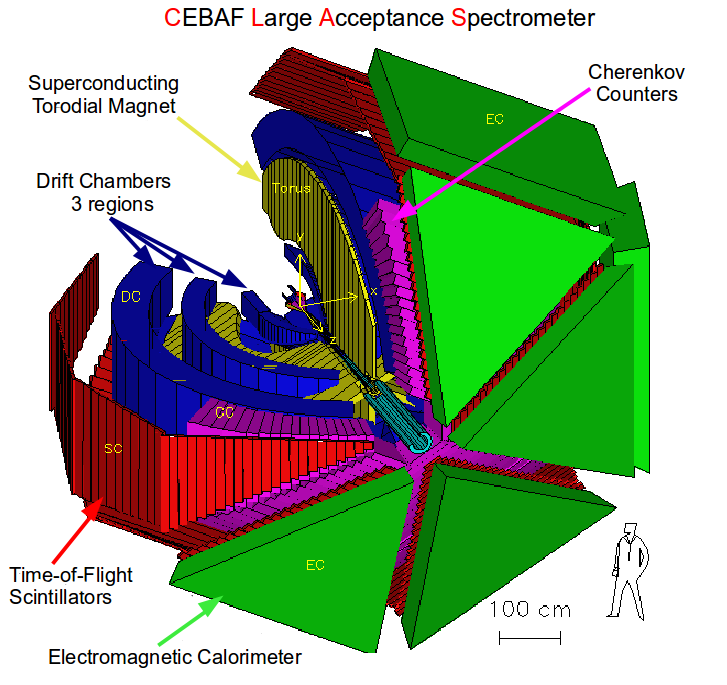
\includegraphics[scale=0.3]{fig/test_clas.png}
\caption{\small\sf Three dimensional representation of the primary CLAS setup represents the geometry and the relative position of each subsystem. From outside, the electromagnetic calorimeter (green), time-of-flight system (red), Cherenkov counters (purple), three drift chamber regions (blue) and the superconducting torus coils (yellow).} 
\label{fig:CLAS}
\end{figure}

CLAS is composed of several subdetectors and two magnets. They are designed to track charged particles at momentum greater than 250 MeV/c. Figure~\ref{fig:CLAS} shows the basic setup of CLAS, ordered with respect to their radial distance from the center:

\begin{itemize}
\item Three regions of Drift Chambers (DC) for tracking of charged particles~\cite{DCref}.
\item Superconducting toroidal magnet which enables the tracking by bending the trajectories.
\item Cherenvkov Counters (CC) to separate electrons from negative pions~\cite{CCref}.
\item Scintillation Counters (SC) to identify hadrons via measuring their Time-Of-Flight (TOF)~\cite{TOFref}.
\item Forward Electromagnetic Calorimeter (EC) to detect showering particles (electrons and photons) and neutrons~\cite{ECref}.
\end{itemize}

In addition to the normal CLAS setup, a forward electromagnetic calorimeter (the inner calorimeter) was installed to improve the photon detection acceptance. Moreover, a 5~T solenoid was placed around the target to shield the detectors close to the beam line -- mostly the inner calorimeter and the RTPC -- from Mollers electrons. The solenoid field is also used to calculate the momentum of the alpha particles from their curvature radius measured by the RTPC.

The first implementation of a RTPC in CLAS have been achieved for the BoNuS experiment~\cite{BONUS} in 200x. The success of this detector for the detection of slow protons motivated the development of this new RTPC. For the channel of interests of our experiments, the recoiled $^{4}He$ nuclei have momentum around (150 or 300 ???) MeV/c, the detection of these particles was the primary motivation for using such design. 

This paper is organized in this way: section $\RNum{2}$ details the design and the internal structure of the RTPC, while section $\RNum{3}$ points the properties of the readout system. The calibration strategies for such detectors will be discussed in section $\RNum{4}$. Finally, performances are discussed in section $\RNum{5}$.

 
\section{Design}

The RTPC is a 200~mm long with a 150~mm diameter time projection chamber. The ionized electrons are drifting outward perpendicularly to the beam direction. These electrons are then amplified by three layers of GEMs and detected on 4.45 by 5~mm pads. As for BoNuS, the RTPC has two detection parts but unlike BoNuS they are part of a single chamber. Each part has independent GEM amplification systems that cover around 80\% of the azimuthal angle. Under the effect of the electromagnetic field, the ionization electrons drift to the readout system on the external shell with a curved trajectory as can be seen in the figure~\ref{fig:RTPC_1_4}.

\begin{figure}[tb]
\centering
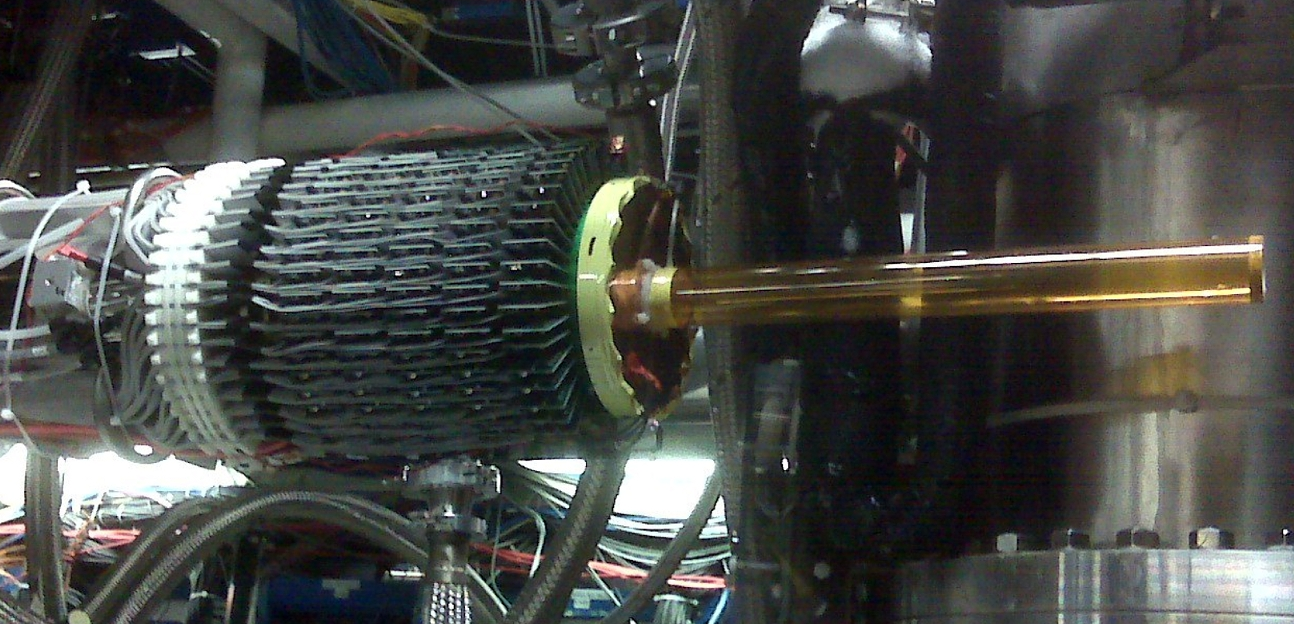
\includegraphics[scale=0.19]{fig/RTPC_exp.png}
\caption[]{\small\sf View of the RTPC ready to be inserted in the solenoid. } 
\label{fig:RTPC2}
\end{figure}

\begin{figure}[tb]
\centering
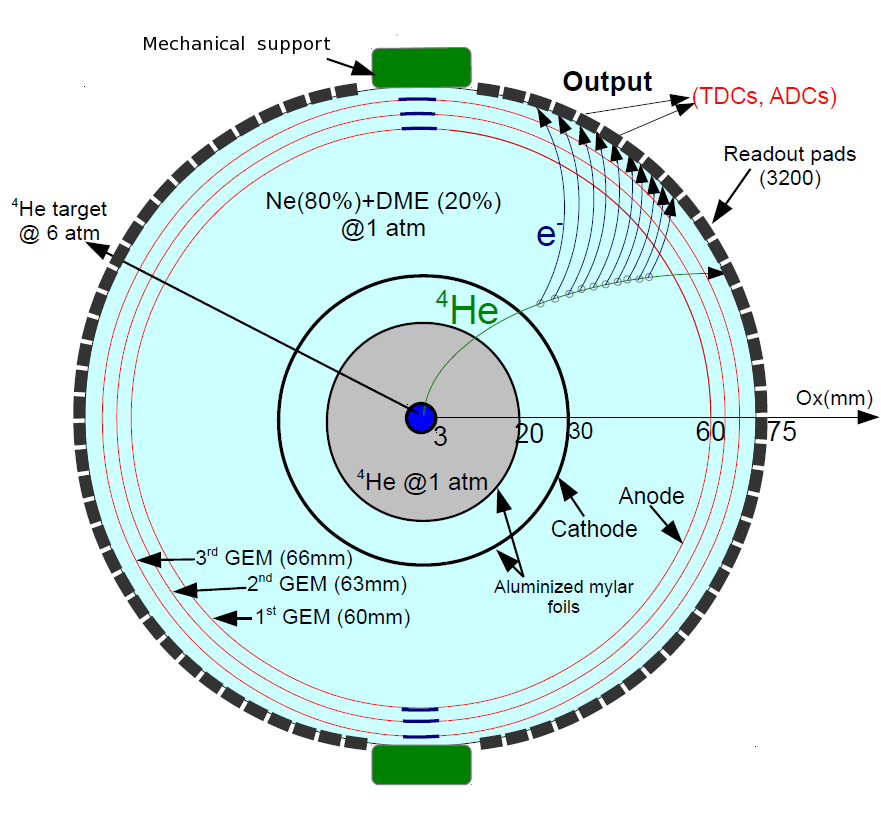
\includegraphics[scale=0.28]{fig/RTPC_1_all.png}
\caption[]{\small\sf Schematic drawing of the RTPC taken on a plane perpendicular to the beam line, see text for description of the elements.} 
\label{fig:RTPC_1_4}
\end{figure} 

As seen in figure~\ref{fig:RTPC2}, the RTPC is composed from the beam axis to the exterior by:\\
\begin{itemize}
\item The target, filled with 5~atm $^4$He, has a 3~mm radius with Kapton walls only 27$\mu$m thick.
\item The first gas gap extends from 3 mm to 20 mm radial distance. It is filled with $^{4}He$ gas at 1~atm. During run, this region is swarmed by Moller electrons induced by the beam, such that filling this region with a light gas like $^{4}He$ minimizes secondary interactions. This region is surrounded by a 4 $\mu$m thick window made of aluminized Mylar and connected to ground. 
\item The gap region extends between 20~mm and 30~mm and is filled with a gas mixture of 80$\%$ Neon and 20$\%$ Dimethyl Ether (DME). This region is surrounded by a 4~$\mu$m thick window made of aluminized Mylar, which serves as the cathode.
\item The drift region is filled with the Ne-DME gas mixture, it extends from the cathode to the first Gas Electron Multiplier(GEM), 60 mm away from the central axis. The electric field in this region is around 500~V/cm (???) and perpendicular to the beam. Field cages are installed at both ends of the detector in this region. Progressive voltage depending on radial position is applied on these to maintain a uniform electric field perpendicular to the beam line at the edges of the RTPC.
\item The GEM system is composed of three GEMs located at radii, 60 mm, 63 mm and 66 mm, they amplify the electrons to make a measurable signal.
\item The readout board has internal radius of 69~mm and collects the charges, preamplifiers are plugged directly on its outer side and are transmitting the signal to the data acquisition electronics.
\end{itemize}
\begin{figure}[tb]
\centering
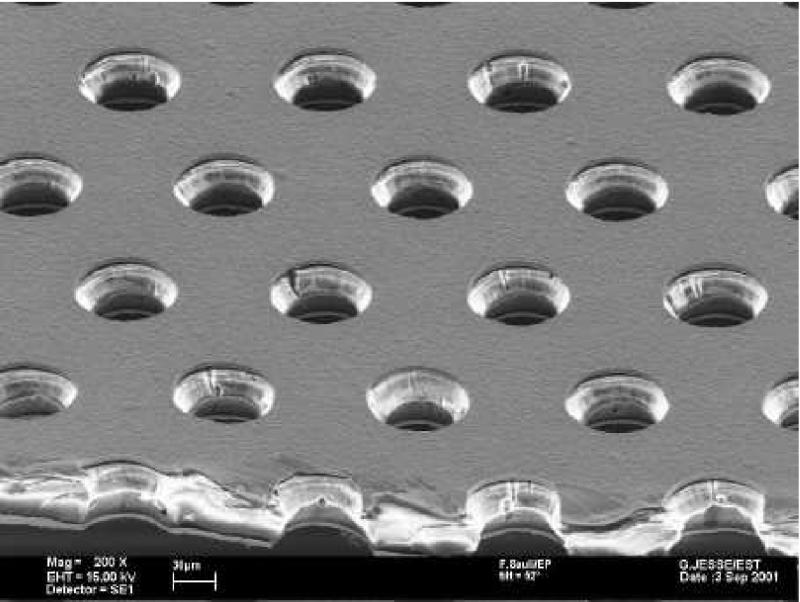
\includegraphics[scale=0.70]{fig/GEM_photo.jpg}
\caption[]{\small\sf A schematic layout of the GEMs system in one module of the RTPC.} 
\label{fig:GEMs}
\end{figure}

The GEM amplification has been mainly chosen for this detector for their flexibility, allowing the curved amplification surface. Also GEM are known to create less sparks than in other gaseous detectors, which is a good thing for the detection of slow nuclei like $^4$He. GEMs are made from an insulator layer (here Kapton) sandwiched between two 5 $\mu$m copper layers. The mesh of each GEM layer is chemically etched with 50$\mu$m diameter holes in double-conical cross section shapes as can be seen in figure~\ref{fig:GEMs}. A potential difference of 400 V is applied between the two copper layers of each GEM creating a very strong electric field in the holes. Such strong fields lead to high ionization from initial electrons and therefore amplification of the signal. Also, a potential difference of 150 V is set between the GEMs to push the amplified electrons toward the readout pads. The gain of each GEM layer is of order 100.\\

\section{Readout System}
The RTPC electron collecting system has 3200 readout pads. These collection elements are located at the end of the amplification region, 69 mm from the central axis.
\begin{figure}[tb]
\centering
%\hspace{-1 cm}
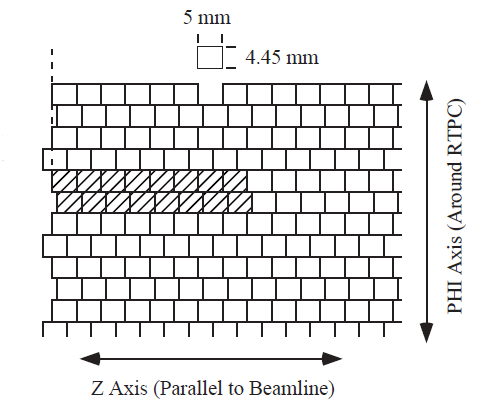
\includegraphics[scale=0.55]{fig/PADs.png}
\caption[]{\small\sf A schematic representation of a part of the readout system. The shaded sixteen pads are a group of pads that are connected to the same pre-amplifier.} 
\label{fig:PADs}
\end{figure}
Figure \ref{fig:PADs} shows a schematic drawing of the size and the alignment configuration of the pads. Each readout pad is 5 mm in length and 4.45 mm in width the shift between the rows allows to reduce aliasing. Each half of the RTPC has 40 rows and 40 columns of pads. The shaded region in the figure~\ref{fig:PADs} shows how pads are grouped to the 16 channels pre-amplifiers. The Time to Digital Converter (TDC) units are 114~ns and indicates the time taken by the electron to drift from the ionization point to the readout board. On the the other side, the charge information is measured in Analog-to-Digital-Converter (ADC) units without specific normalization. 

Missing items in description:

Detail the electronic setup: Andrea ? or other Italians?

The gas mixture choice: ???

Discuss HV setting: ???

\section{Calibration}
Two quantities are recorded for each detected electron at the readout board, time (TDCs) and signal amplitude (ADCs) (/!\\ are those amplitude or charge preamps ???). The timing information provides trajectory determination resulting in momentum per unit charge measurement. Going from a collection of the TDCs to a momentum measurement requires good knowledge of the drift speed and paths followed by the electrons released in the gas. The recorded ADCs give the deposited energy per unit of length ($\small{\frac{dE}{dX}}$) which, together with the momentum calculated from the trajectory, enables particle identification.


\subsection{Drift Speed Parametrization}

We can measure the drift speed using the tracks detected in the RTPC, in figure \ref{fig:RTPC_signals} we represent a typical $^{4}He$ track (in green). After it causes ionization in the drift region, the released electrons (in black) drift to the detection plane under the effect of the electric field. The electrons released close to the cathode take the most time to reach the readout pads while the geometrical symmetry insure they always travel the same distance. So by identifying the maximum TDC measured, we can infer the drift speed of the electrons in the RTPC.\\

\begin{figure}[tb]
\centering
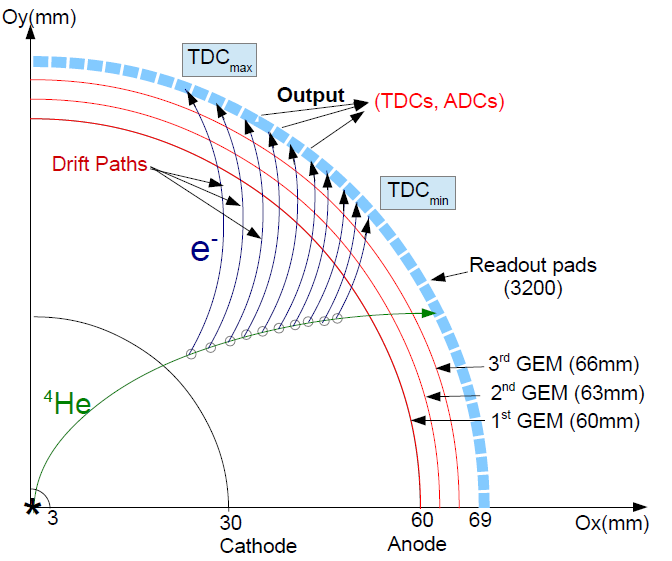
\includegraphics[scale=0.35]{fig/RTPC_2.png}
\caption[]{\small\sf A schematic drawing of a $^{4}He$ track (in green) traversing the drift region, with the drift paths followed by the electrons (in black). } 
\label{fig:RTPC_signals}
\end{figure}

We first measure the drift speed along the 200 mm RTPC's length to take into account variations in the electric and magnetic field, some of which are known (see figure \ref{fig:B_MAP}) some might be due to slight shifts in the geometry. We verified this by looking at the TDC profile generated in the chamber by all our tracks (see figure \ref{fig:TDC_profile}). The time profile of registered hits clearly show the dropping edge expected from the geometrical considerations previously mentioned. We define a value named $TDC_{Max/2}$ at which the dropping edge passes half the maximum number of hits in the histogram, this value is inversely proportional to the drift speed. The result can be seen in figure \ref{fig:RunNumber_61551_TDCmax_Zslice} showing the dependence of drift speed with position along the beam line axis in the chamber. 

\begin{figure}[tb]
\centering
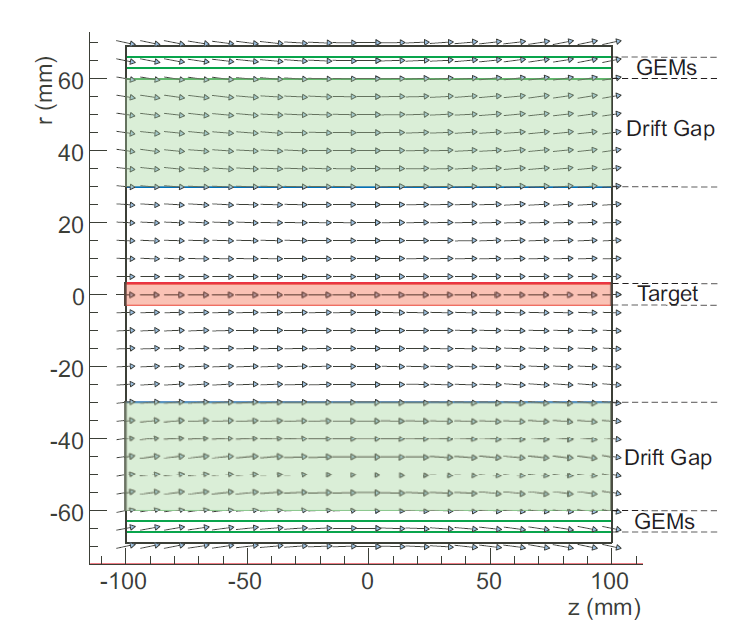
\includegraphics[scale=0.35]{fig/B_MAP.png}
\caption[]{\small\sf Schematic draw in of the solenoid magnetic vectors inside the RTPC. In this draw, r is the radial distance from the target's axis and z is the longitudinal position along the RTPC with its center at zero.} 
\label{fig:B_MAP}
\end{figure}

\begin{figure}[tb]
\centering
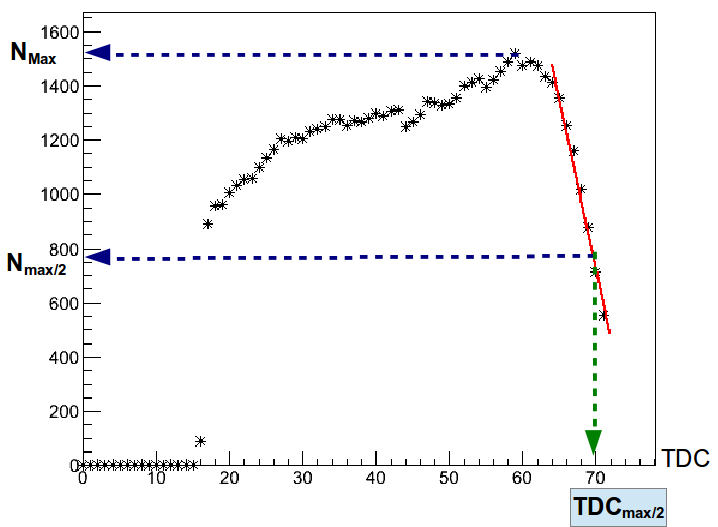
\includegraphics[scale=0.40]{fig/TDC_profile.png}
\caption[]{\small\sf Time profile of the collected hits in one experimental run. } 
\label{fig:TDC_profile}
\end{figure}

\begin{figure}[tb]
\centering
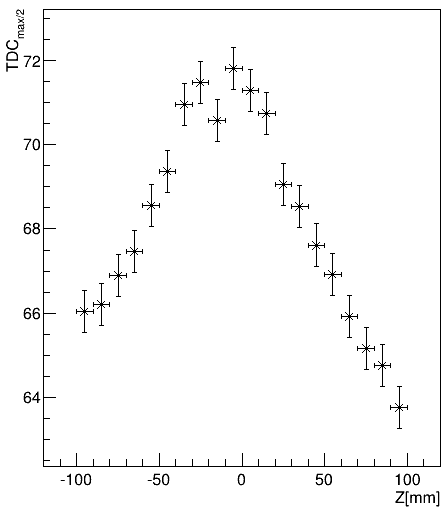
\includegraphics[scale=0.4]{fig/RunNumber_61551_TDCmax_Zslice.png}
\caption[]{\small\sf Time profile distribution for the collected hits in one experimental run. } 
\label{fig:RunNumber_61551_TDCmax_Zslice}
\end{figure}

Due to the non perfect experimental conditions and in particular changes in the gas proportions, the drift speed might also change over the 3 months run. Figure \ref{fig:Drift_run_number_1} shows the $TDC_{Max/2}$ values for individual runs (approximately 2 hours long). We observe a significant variation over time that we parametrized with a fit in order to take it into account in the track reconstruction code. Dealing with such situation is possible by adapting the right drift speed to the electrons as a function of geometry and time (we did not see any correlation between the effects). These functions were extracted for our entire data sets and implemented in the reconstructions code.

\begin{figure}[tb]
\hspace*{-1.8cm}
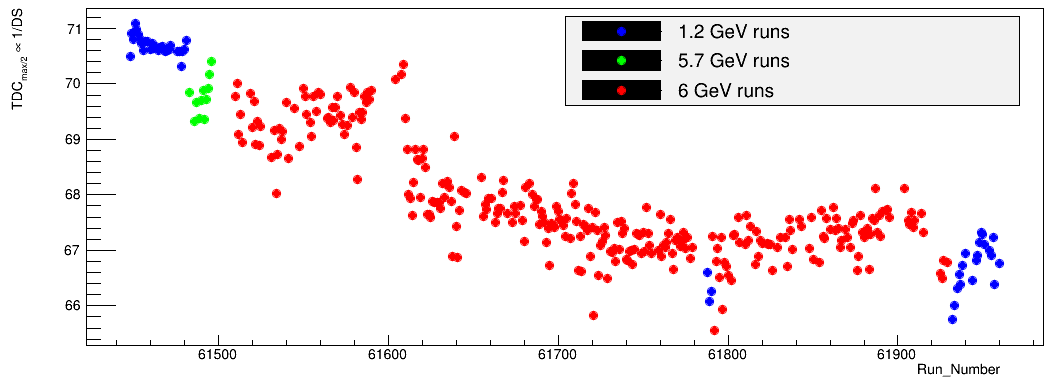
\includegraphics[scale=0.28]{fig/Drift_run_number_1.png}
\caption[]{\small\sf $TDC_{Nbmax/2}$ versus the experimental run numbers (time). } 
\label{fig:Drift_run_number_1}
\end{figure}

   
\subsection{Drift Paths Parametrization}

The drift path is the trajectory which an electron follows in the gas. The standard software to calculate drift paths is the MAGBOLTZ program ~\cite{MAGBOLTZ}. For its calculations, MAGBOLTZ needs to know the detector's geometry, the exact composition of the gas mixture and of course the electric and the magnetic fields. We used such calculations as a first calibration, but as can be seen with the drift speed, conditions are far from stable in the chamber. Moreover, because we use of a thin foil as a cathode, the geometry knowledge is limited to a millimeter precision. These problems, already encountered for the BoNuS RTPC calibration (ref), have motivated the acquisition of specific calibration runs. These are taken with lower energy electron beam (1.20 and 1.27 GeV) to enhance the cross section of the elastic process ($e ^{4}He \rightarrow e ^{4}He$). In this process the knowledge of the electron kinematic gives us the helium nuclei kinematic and therefore allow us to calibrate our drift paths independently of our knowledge of the exact conditions in the chamber.

The drift paths' parametrization is possible using identified elastic events from our experiment and simulate copy of them in a GEANT4 simulation~\cite{GEANT4}. Then by comparing the GEANT4 calculated position of the helium nuclei to the list of hits effectively measured in the chamber, we can reconstruct the electrons drift path in the RTPC. However, because of the magnetic field, the drift paths are not linear. So to perform the extraction, we make a first assumption of a linear dependence between the radius of emission and the TDC of detection and then refine our result. As it happens, the curvature is minimal and this process converge already on the second iteration. Here are the step of the extraction procedure (we work in a polar coordinate system ($R$,$\phi$), $\Delta\phi$ being the difference between the $\phi$ of the pad measuring a hit and the $\phi$ of the simulated helium):

\begin{figure}[tb]
\centering
%\hspace{-0.95cm}
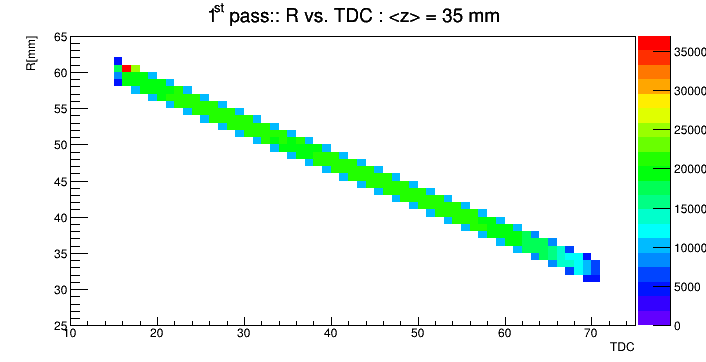
\includegraphics[scale=0.37]{fig/R_correlation.png}
\caption[]{\small\sf R versus TDC distribution for the simulated hits locating in a single $z$ bin. The maximum $R$ equals 60 mm (close to the anode) at minimum TDCs (Trigger time is 15), and minimum R equals 30 mm (close to the cathode) at maximum TDCs ($\sim75$).}
\label{fig:R_correlation}
\end{figure} 

\begin{itemize}
\item The linear assumption between R and time(TDC) is necessary to link the generated hits from GEANT4 to physical hits. Figure \ref{fig:R_correlation} shows our initial $R$ versus TDC. \\
\item For these selected hits, we look at $\Delta\phi$ ($\Delta \phi$ = $\phi_{sim.}$ - $\phi_{hit\_pad}$) versus TDC. We clearly obtain a correlation shown in figure~\ref{fig:1st_pass_delta_phi}. This $\Delta \phi$ change with TDC shows the drift in $phi$ of the electrons due to the Lorentz angle. \\

\begin{figure}[tb]
\centering
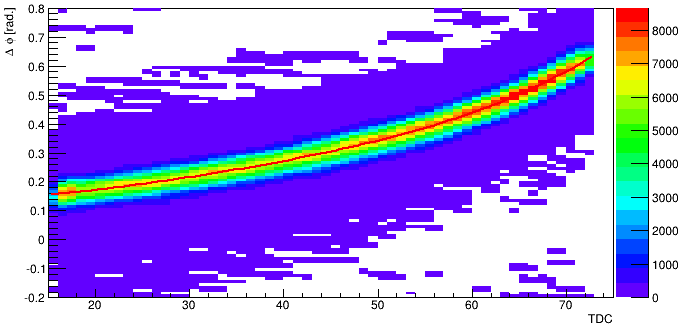
\includegraphics[scale=0.37]{fig/1st_pass_delta_phi.png}
\caption[]{\small\sf $\Delta \phi$ versus TDC distribution for the simulated hits locating in one slice centered at 35 mm.}
\label{fig:1st_pass_delta_phi}
\end{figure} 

\item Using this first measurement, we can calculate a new correlation between $R$ and TDC. The result, shown in figure~\ref{fig:R_TDC}, is very close to linear explaining the fast convergence of our procedure. \\

\begin{figure}[tb]
\centering
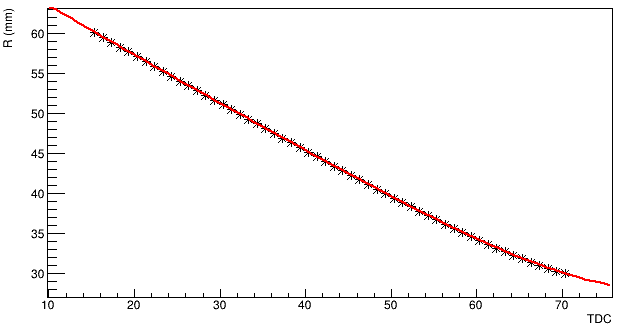
\includegraphics[scale=0.37]{fig/R_TDC.png}
\caption[]{\small\sf The calculated R versus the time is corrected by the parameters of $\Delta \phi$ from the first pass.}
\label{fig:R_TDC}
\end{figure}

\item In the second pass, we associate simulated helium positions to physical hits according to their calculated correlation and obtain new $\Delta \phi$ distributions.\\
\item We finally parametrize the $\Delta\phi$ distributions with a fit as can be seen in figure~\ref{fig:DELTA_PHI_TDC}, which shows the final $\Delta \phi$ versus TDC with a red line representing our drift paths fit.
\end{itemize}

\begin{figure}[tb]
\centering
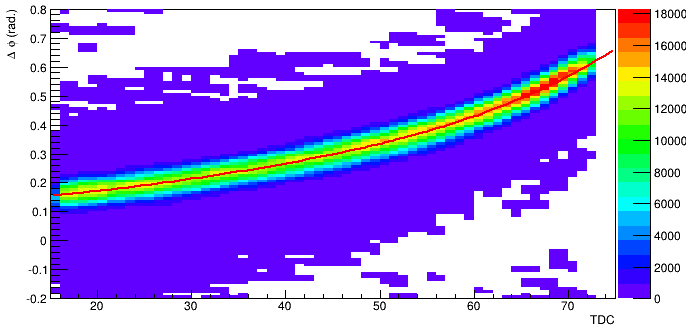
\includegraphics[scale=0.37]{fig/DELTA_PHI_TDC.png}
\caption[]{\small\sf $\Delta \phi$ versus TDC distribution in the second pass for the slice centered at 35 mm longitudinal position along the RTPC. The red line represents the final drift paths in this slice.}
\label{fig:DELTA_PHI_TDC}
\end{figure}

To verify the stability of the drift paths, this procedure was carried out using both the 1.204 GeV data set from the beginning of the run period and the 1.269 GeV data from the end of the run period. As a result, we found very similar drift paths and reached the conclusion that whatever changed in the setting affected only the drift speed.

\subsection{Gain Calibration}

The parametrization of the drift speed and the drift paths were carried out using only the TDCs, gain calibration goal is to equalize the gains in ADC/MeV over the full RTPC. The gain of each pad is the ratio between the actual deposited energy and the registered ADC value. We identified three different methods to extract such gains. The first is to compare the experimental energy deposit to the expected value calculated from Bethe-Block formula (ref). The second method is to compare the experimental ADCs to the energy deposited in GEANT4 by simulated tracks (using the same elastic events than for the drift paths calibration). In the third method, the ADCs of each pad is compared to the ADCs of the other pads inside each track.

(Detail of 1st method: Nathan)

To perform the second method it requires a very good GEANT4 simulation including drift paths, but also drift and amplification spreads of the charges before reaching the pad, so that the simulated hits match the experimental ones. Moreover, the simulation has to match the data acquisition (DAQ) features that can lead to cutting out hits. After setting the simulation properly, we can compare simulation to data on an event by event basis as in figure~\ref{fig:EVENT_adc_tdc}. In this step, the gain for each pad is defined as the ratio of the measured ADCs to the simulated deposited energy.

(Detail of 3rd method: Mohammad)

\begin{figure}[tb]
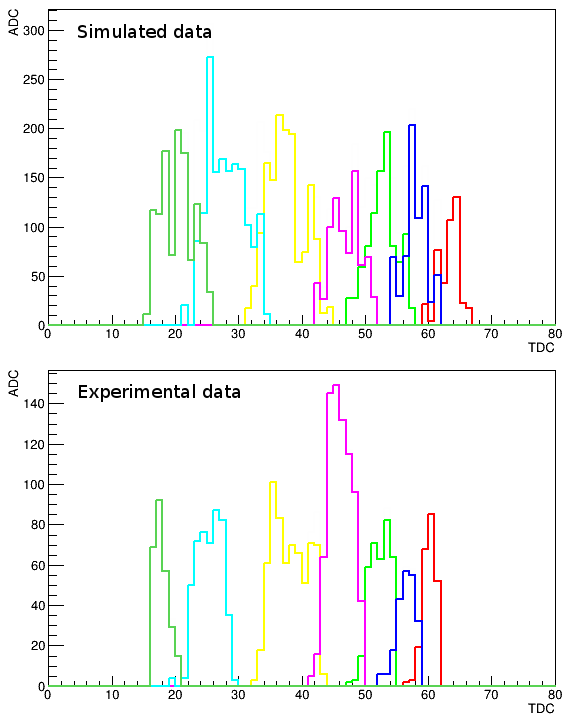
\includegraphics[scale=0.350]{fig/EVENT_adc_tdc.png}
\caption[]{\small\sf Simulated (upper) and experimental (lower) ADCs and TDCs distributions of a track. The colors indicate the pads, same color in top and bottom indicate that they are the same pad.}
\label{fig:EVENT_adc_tdc}
\end{figure}

\begin{figure}[tb]
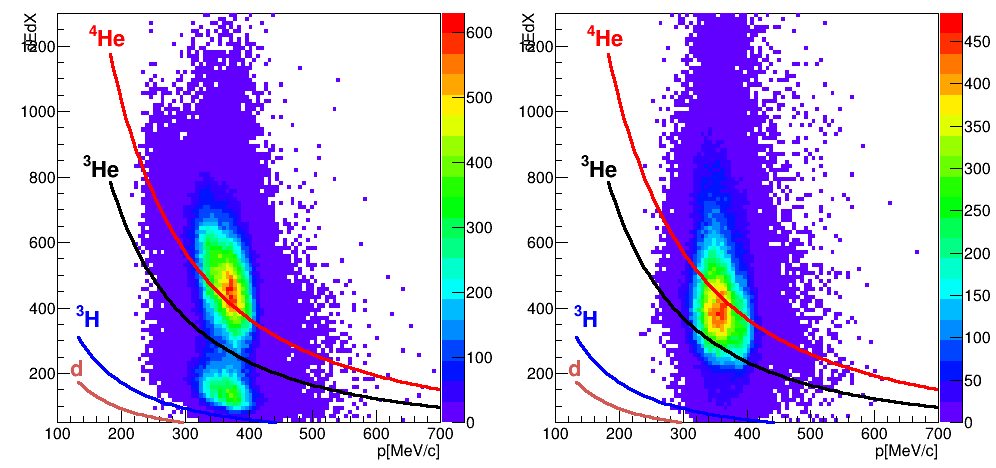
\includegraphics[scale=0.26]{fig/dedx_p_exp_1st.png}
\caption[]{\small\sf $\small{\frac{dE}{dX}}$ vs. p distribution for the left half of the RTPC (left) and for the right half (right). Here, $\small{\frac{dE}{dX}}$ is calculated using the gains of the first method. The lines are theoretical expectations from Bethe-Bloch formula for $^4$He, $^3$He, $^3$H and $^2$H (d).}
\label{fig:dedx_p_exp_1st}
\end{figure}

\begin{figure}[tb]
\centering
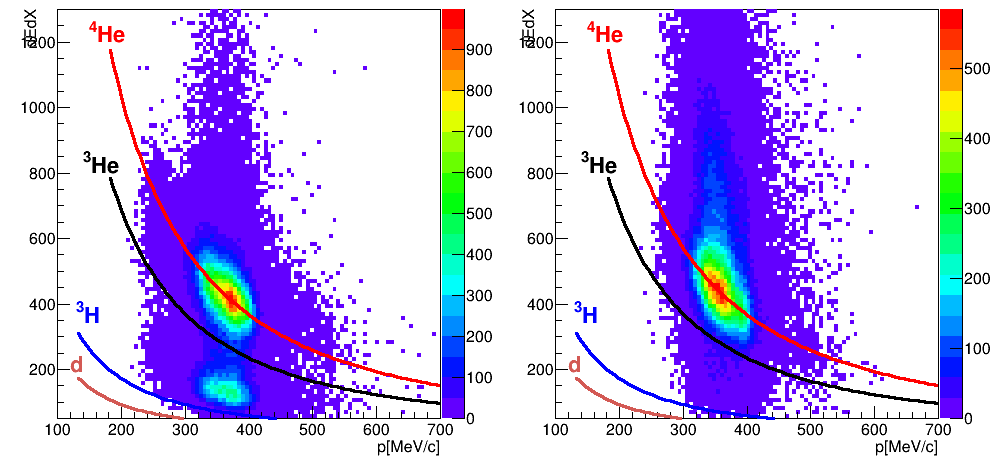
\includegraphics[scale=0.26]{fig/dedx_p_exp_2nd.png}
\caption[]{\small\sf $\small{\frac{dE}{dX}}$ vs. p distribution for the left half of the RTPC (left) and for the right half (right). Here, $\small{\frac{dE}{dX}}$ is calculated using the gains of the second method. The lines are theoretical expectations from Bethe-Bloch formula for $^4$He, $^3$He, $^3$H and $^2$H (d).}
\label{fig:dedx_p_exp_2nd}
\end{figure}

A set of gains has been extracted from each method, in figure~\ref{fig:dedx_p_exp_1st}, we have $\small{\frac{dE}{dX}}$ calculated using the first method's gains, while in Figure~\ref{fig:dedx_p_exp_2nd} we use the second method's gains. From these, we concluded that the gains of the second method match best the theoretical lines. This is not surprising since calibrating with full tracks leads to mixing the gains from the different pads. So it seems that even with several iterations, we could not decipher properly the effects of individual pads with this method.

\subsection{Noise Rejection}

(To be written by Nathan) 

\begin{figure}[tb]
\hspace{-0.4cm}
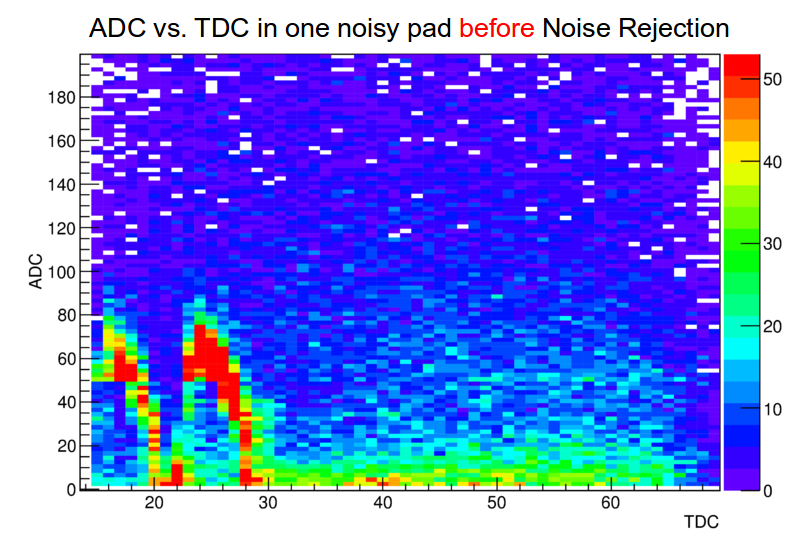
\includegraphics[scale=0.27]{fig/noisy_pad_before_rejection.png}
\caption[]{\small\sf }
\label{fig:noisy_pad_before_rejection}
\end{figure}

\begin{figure}[tb]
\hspace{-0.4cm}
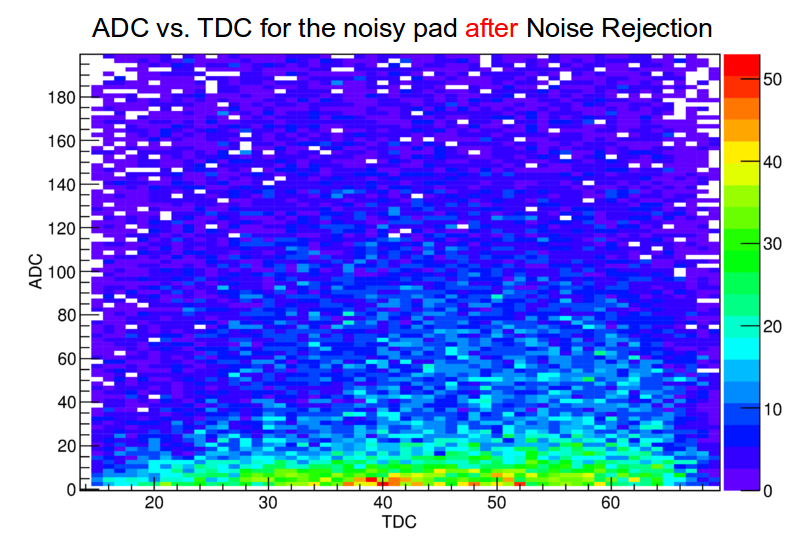
\includegraphics[scale=0.27]{fig/noisy_pad_after_rejection.png}
\caption[]{\small\sf }
\label{fig:noisy_pad_after_rejection}
\end{figure}

\section{Track Reconstruction}

In order to reconstruct tracks we first select good hits. This means rejecting out-of-time hits and hits linked to the electronic noise. The second step is space-reconstructing the hits using the extracted drift speed and drift path parameters. For each registered hit, we calculate a position of emission from the recorded time (TDC) and the position of the recording pad. The third step is to create chains of hits. The maximum distance between two close adjacent hits has to be less than 10.5 mm to chain them, this roughly correspond to neighbors and next to neighbors. Then, we fit the chains that have a minimum of 10 hits. We make the fit in two iterations, first, all the hits of the chain together with the beam line are fitted with a helix. For the second iteration, the hits that are 5 mm or farther from the first fit are excluded.

For the energy deposit, $\frac{dE}{dx}$ is calculated in this way:
\begin{equation}
 \left\langle \frac{dE}{dX} \right\rangle= \frac{\sum\limits_{i} \frac{ADC_{i}}{Gi}}{vtl}
\end{equation}
Where the sum runs over all the hits of the track and $G_{i}$ is the gain of the associated pad. The $vtl$ is the visible track length in the active drift volume. 

(We need some performance studies here: Mohammad)

\section{Conclusion}

(TBD)

\begin{thebibliography}{}
\bibitem{CLASref}
B.A. Mecking et al., "The CEBAF large acceptance spectrometer", Nucl. Inst. and Meth. A 503, 513 (2003).

\bibitem{proposal}
K.Hafidi et al., "Deeply virtual Comton scattering off 4He", Jlab proposal to PAC33 (2007).
\bibitem{DCref}
M.D. Mestayer et al., "The CLAS drift chamber System", Nucl. Inst. and Meth. A 449, 81 (2000)

\bibitem{CCref}
G. Adams et al., "The CLAS Cerenkov detector", Nucl. Inst. and Meth. A 465, 414 (2001).

\bibitem{TOFref}E.S. Smith et al., "The time-of-flight system for CLAS", Nucl. Inst. and Meth. A 432, 265 (1999).

\bibitem{ECref}
M. Amarian et al., "The CLAS forward electromagnetic calorimeter", Nucl. Inst. and Meth. A 460, 239 (2001). 

\bibitem{BONUS}
S. Tkachenko et al., "Measurement of the nearly free neutron structure function using spectator tagging in inelastic $^{2}H(e,e'p)X$ scattering with CLAS",	Phys. Rev. C 89, 045206 (2014).

\bibitem{MAGBOLTZ}
S. Biagi, "Monte Carlo simulation of electron drift and diffusion in counting gases under the influence of electric and magnetic fields", Nucl. Inst. and Meth. in Phy. Res. A, vol. 421, pp. 234-240, 1999.

\bibitem{GEANT4}
http://geant4.cern.ch

\end{thebibliography}

\end{document}

